% Created by tikzDevice version 0.12 on 2019-01-31 15:22:33
% !TEX encoding = UTF-8 Unicode
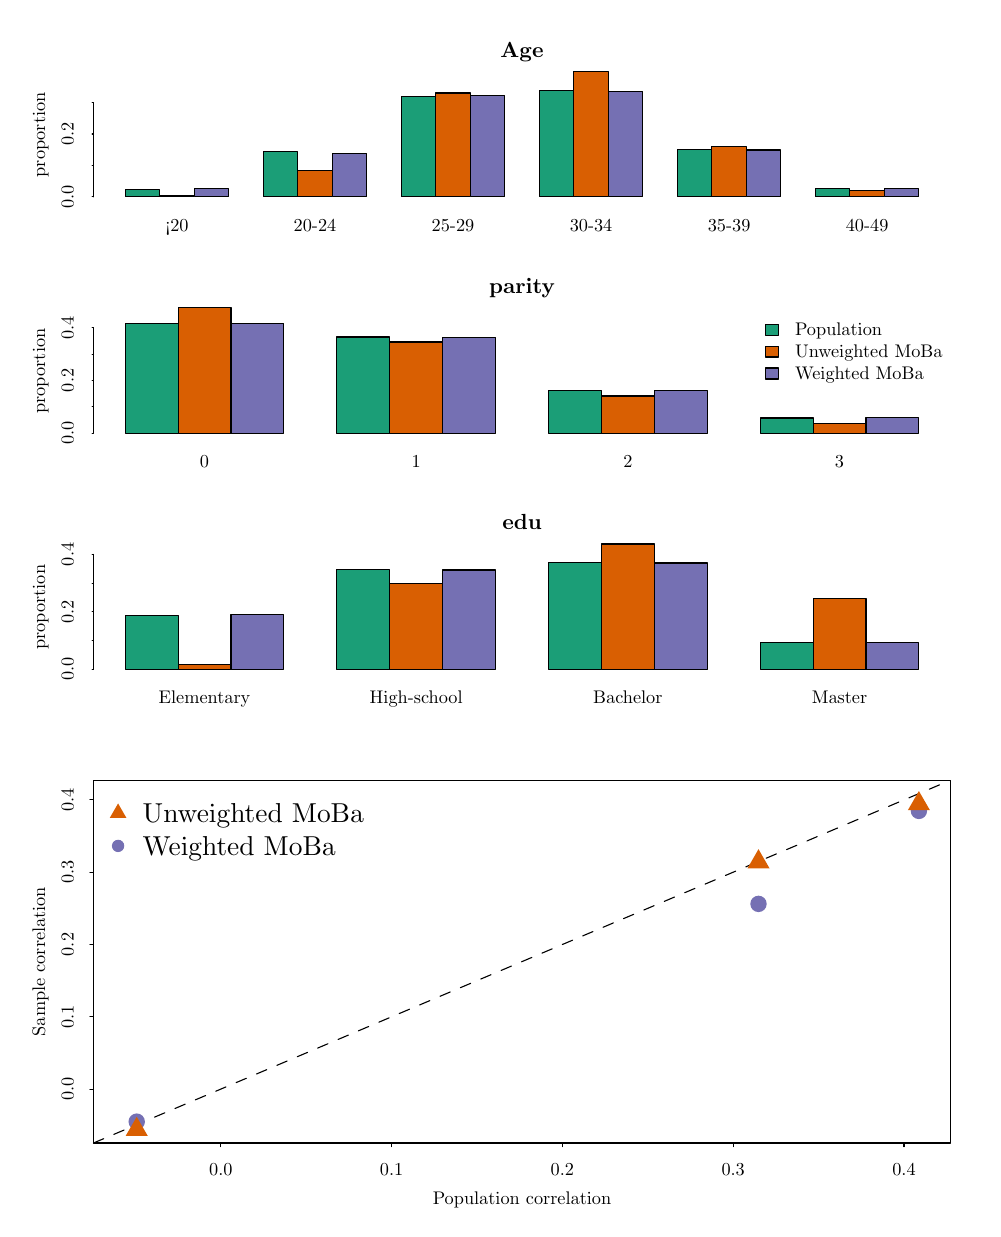
\begin{tikzpicture}[x=1pt,y=1pt]
\definecolor{fillColor}{RGB}{255,255,255}
\path[use as bounding box,fill=fillColor,fill opacity=0.00] (0,0) rectangle (341.43,426.79);
\begin{scope}
\path[clip] (  0.00,341.43) rectangle (341.43,426.79);
\definecolor{drawColor}{RGB}{0,0,0}
\definecolor{fillColor}{RGB}{27,158,119}

\path[draw=drawColor,line width= 0.4pt,line join=round,line cap=round,fill=fillColor] ( 35.23,365.65) rectangle ( 47.70,368.25);
\definecolor{fillColor}{RGB}{217,95,2}

\path[draw=drawColor,line width= 0.4pt,line join=round,line cap=round,fill=fillColor] ( 47.70,365.65) rectangle ( 60.17,366.30);
\definecolor{fillColor}{RGB}{117,112,179}

\path[draw=drawColor,line width= 0.4pt,line join=round,line cap=round,fill=fillColor] ( 60.17,365.65) rectangle ( 72.64,368.54);
\definecolor{fillColor}{RGB}{27,158,119}

\path[draw=drawColor,line width= 0.4pt,line join=round,line cap=round,fill=fillColor] ( 85.11,365.65) rectangle ( 97.58,382.00);
\definecolor{fillColor}{RGB}{217,95,2}

\path[draw=drawColor,line width= 0.4pt,line join=round,line cap=round,fill=fillColor] ( 97.58,365.65) rectangle (110.05,375.24);
\definecolor{fillColor}{RGB}{117,112,179}

\path[draw=drawColor,line width= 0.4pt,line join=round,line cap=round,fill=fillColor] (110.05,365.65) rectangle (122.52,381.42);
\definecolor{fillColor}{RGB}{27,158,119}

\path[draw=drawColor,line width= 0.4pt,line join=round,line cap=round,fill=fillColor] (134.99,365.65) rectangle (147.46,401.98);
\definecolor{fillColor}{RGB}{217,95,2}

\path[draw=drawColor,line width= 0.4pt,line join=round,line cap=round,fill=fillColor] (147.46,365.65) rectangle (159.93,403.17);
\definecolor{fillColor}{RGB}{117,112,179}

\path[draw=drawColor,line width= 0.4pt,line join=round,line cap=round,fill=fillColor] (159.93,365.65) rectangle (172.40,402.35);
\definecolor{fillColor}{RGB}{27,158,119}

\path[draw=drawColor,line width= 0.4pt,line join=round,line cap=round,fill=fillColor] (184.87,365.65) rectangle (197.34,403.95);
\definecolor{fillColor}{RGB}{217,95,2}

\path[draw=drawColor,line width= 0.4pt,line join=round,line cap=round,fill=fillColor] (197.34,365.65) rectangle (209.81,410.95);
\definecolor{fillColor}{RGB}{117,112,179}

\path[draw=drawColor,line width= 0.4pt,line join=round,line cap=round,fill=fillColor] (209.81,365.65) rectangle (222.28,403.87);
\definecolor{fillColor}{RGB}{27,158,119}

\path[draw=drawColor,line width= 0.4pt,line join=round,line cap=round,fill=fillColor] (234.75,365.65) rectangle (247.22,382.67);
\definecolor{fillColor}{RGB}{217,95,2}

\path[draw=drawColor,line width= 0.4pt,line join=round,line cap=round,fill=fillColor] (247.22,365.65) rectangle (259.69,383.70);
\definecolor{fillColor}{RGB}{117,112,179}

\path[draw=drawColor,line width= 0.4pt,line join=round,line cap=round,fill=fillColor] (259.69,365.65) rectangle (272.16,382.60);
\definecolor{fillColor}{RGB}{27,158,119}

\path[draw=drawColor,line width= 0.4pt,line join=round,line cap=round,fill=fillColor] (284.63,365.65) rectangle (297.10,368.54);
\definecolor{fillColor}{RGB}{217,95,2}

\path[draw=drawColor,line width= 0.4pt,line join=round,line cap=round,fill=fillColor] (297.10,365.65) rectangle (309.57,368.03);
\definecolor{fillColor}{RGB}{117,112,179}

\path[draw=drawColor,line width= 0.4pt,line join=round,line cap=round,fill=fillColor] (309.57,365.65) rectangle (322.04,368.61);
\end{scope}
\begin{scope}
\path[clip] (  0.00,  0.00) rectangle (341.43,426.79);
\definecolor{drawColor}{RGB}{0,0,0}

\node[text=drawColor,anchor=base,inner sep=0pt, outer sep=0pt, scale=  0.66] at ( 53.94,353.31) {<20};

\node[text=drawColor,anchor=base,inner sep=0pt, outer sep=0pt, scale=  0.66] at (103.82,353.31) {20-24};

\node[text=drawColor,anchor=base,inner sep=0pt, outer sep=0pt, scale=  0.66] at (153.70,353.31) {25-29};

\node[text=drawColor,anchor=base,inner sep=0pt, outer sep=0pt, scale=  0.66] at (203.58,353.31) {30-34};

\node[text=drawColor,anchor=base,inner sep=0pt, outer sep=0pt, scale=  0.66] at (253.46,353.31) {35-39};

\node[text=drawColor,anchor=base,inner sep=0pt, outer sep=0pt, scale=  0.66] at (303.34,353.31) {40-49};
\end{scope}
\begin{scope}
\path[clip] (  0.00,341.43) rectangle (341.43,426.79);
\definecolor{drawColor}{RGB}{0,0,0}

\node[text=drawColor,anchor=base,inner sep=0pt, outer sep=0pt, scale=  0.79] at (178.64,416.14) {\bfseries Age};

\node[text=drawColor,rotate= 90.00,anchor=base,inner sep=0pt, outer sep=0pt, scale=  0.66] at (  6.34,388.07) {proportion};
\end{scope}
\begin{scope}
\path[clip] (  0.00,  0.00) rectangle (341.43,426.79);
\definecolor{drawColor}{RGB}{0,0,0}

\path[draw=drawColor,line width= 0.4pt,line join=round,line cap=round] ( 23.76,365.65) -- ( 23.76,399.70);

\path[draw=drawColor,line width= 0.4pt,line join=round,line cap=round] ( 23.76,365.65) -- ( 23.30,365.65);

\path[draw=drawColor,line width= 0.4pt,line join=round,line cap=round] ( 23.76,377.00) -- ( 23.30,377.00);

\path[draw=drawColor,line width= 0.4pt,line join=round,line cap=round] ( 23.76,388.35) -- ( 23.30,388.35);

\path[draw=drawColor,line width= 0.4pt,line join=round,line cap=round] ( 23.76,399.70) -- ( 23.30,399.70);

\node[text=drawColor,rotate= 90.00,anchor=base,inner sep=0pt, outer sep=0pt, scale=  0.66] at ( 16.63,365.65) {0.0};

\node[text=drawColor,rotate= 90.00,anchor=base,inner sep=0pt, outer sep=0pt, scale=  0.66] at ( 16.63,388.35) {0.2};
\end{scope}
\begin{scope}
\path[clip] (  0.00,256.07) rectangle (341.43,341.43);
\definecolor{drawColor}{RGB}{0,0,0}
\definecolor{fillColor}{RGB}{27,158,119}

\path[draw=drawColor,line width= 0.4pt,line join=round,line cap=round,fill=fillColor] ( 35.23,280.29) rectangle ( 54.35,320.00);
\definecolor{fillColor}{RGB}{217,95,2}

\path[draw=drawColor,line width= 0.4pt,line join=round,line cap=round,fill=fillColor] ( 54.35,280.29) rectangle ( 73.47,325.59);
\definecolor{fillColor}{RGB}{117,112,179}

\path[draw=drawColor,line width= 0.4pt,line join=round,line cap=round,fill=fillColor] ( 73.47,280.29) rectangle ( 92.59,319.96);
\definecolor{fillColor}{RGB}{27,158,119}

\path[draw=drawColor,line width= 0.4pt,line join=round,line cap=round,fill=fillColor] (111.71,280.29) rectangle (130.84,315.00);
\definecolor{fillColor}{RGB}{217,95,2}

\path[draw=drawColor,line width= 0.4pt,line join=round,line cap=round,fill=fillColor] (130.84,280.29) rectangle (149.96,313.19);
\definecolor{fillColor}{RGB}{117,112,179}

\path[draw=drawColor,line width= 0.4pt,line join=round,line cap=round,fill=fillColor] (149.96,280.29) rectangle (169.08,314.87);
\definecolor{fillColor}{RGB}{27,158,119}

\path[draw=drawColor,line width= 0.4pt,line join=round,line cap=round,fill=fillColor] (188.20,280.29) rectangle (207.32,295.59);
\definecolor{fillColor}{RGB}{217,95,2}

\path[draw=drawColor,line width= 0.4pt,line join=round,line cap=round,fill=fillColor] (207.32,280.29) rectangle (226.44,293.68);
\definecolor{fillColor}{RGB}{117,112,179}

\path[draw=drawColor,line width= 0.4pt,line join=round,line cap=round,fill=fillColor] (226.44,280.29) rectangle (245.56,295.67);
\definecolor{fillColor}{RGB}{27,158,119}

\path[draw=drawColor,line width= 0.4pt,line join=round,line cap=round,fill=fillColor] (264.68,280.29) rectangle (283.80,285.74);
\definecolor{fillColor}{RGB}{217,95,2}

\path[draw=drawColor,line width= 0.4pt,line join=round,line cap=round,fill=fillColor] (283.80,280.29) rectangle (302.92,283.88);
\definecolor{fillColor}{RGB}{117,112,179}

\path[draw=drawColor,line width= 0.4pt,line join=round,line cap=round,fill=fillColor] (302.92,280.29) rectangle (322.04,285.84);
\end{scope}
\begin{scope}
\path[clip] (  0.00,  0.00) rectangle (341.43,426.79);
\definecolor{drawColor}{RGB}{0,0,0}

\node[text=drawColor,anchor=base,inner sep=0pt, outer sep=0pt, scale=  0.66] at ( 63.91,267.95) {0};

\node[text=drawColor,anchor=base,inner sep=0pt, outer sep=0pt, scale=  0.66] at (140.40,267.95) {1};

\node[text=drawColor,anchor=base,inner sep=0pt, outer sep=0pt, scale=  0.66] at (216.88,267.95) {2};

\node[text=drawColor,anchor=base,inner sep=0pt, outer sep=0pt, scale=  0.66] at (293.36,267.95) {3};
\end{scope}
\begin{scope}
\path[clip] (  0.00,256.07) rectangle (341.43,341.43);
\definecolor{drawColor}{RGB}{0,0,0}

\node[text=drawColor,anchor=base,inner sep=0pt, outer sep=0pt, scale=  0.79] at (178.64,330.78) {\bfseries parity};

\node[text=drawColor,rotate= 90.00,anchor=base,inner sep=0pt, outer sep=0pt, scale=  0.66] at (  6.34,302.71) {proportion};
\end{scope}
\begin{scope}
\path[clip] (  0.00,  0.00) rectangle (341.43,426.79);
\definecolor{drawColor}{RGB}{0,0,0}

\path[draw=drawColor,line width= 0.4pt,line join=round,line cap=round] ( 23.76,280.29) -- ( 23.76,318.36);

\path[draw=drawColor,line width= 0.4pt,line join=round,line cap=round] ( 23.76,280.29) -- ( 23.30,280.29);

\path[draw=drawColor,line width= 0.4pt,line join=round,line cap=round] ( 23.76,289.81) -- ( 23.30,289.81);

\path[draw=drawColor,line width= 0.4pt,line join=round,line cap=round] ( 23.76,299.32) -- ( 23.30,299.32);

\path[draw=drawColor,line width= 0.4pt,line join=round,line cap=round] ( 23.76,308.84) -- ( 23.30,308.84);

\path[draw=drawColor,line width= 0.4pt,line join=round,line cap=round] ( 23.76,318.36) -- ( 23.30,318.36);

\node[text=drawColor,rotate= 90.00,anchor=base,inner sep=0pt, outer sep=0pt, scale=  0.66] at ( 16.63,280.29) {0.0};

\node[text=drawColor,rotate= 90.00,anchor=base,inner sep=0pt, outer sep=0pt, scale=  0.66] at ( 16.63,299.32) {0.2};

\node[text=drawColor,rotate= 90.00,anchor=base,inner sep=0pt, outer sep=0pt, scale=  0.66] at ( 16.63,318.36) {0.4};
\end{scope}
\begin{scope}
\path[clip] ( 23.76,279.83) rectangle (333.51,325.59);
\definecolor{drawColor}{RGB}{0,0,0}
\definecolor{fillColor}{RGB}{27,158,119}

\path[draw=drawColor,line width= 0.4pt,line join=round,line cap=round,fill=fillColor] (266.61,319.65) rectangle (271.36,315.69);
\definecolor{fillColor}{RGB}{217,95,2}

\path[draw=drawColor,line width= 0.4pt,line join=round,line cap=round,fill=fillColor] (266.61,311.73) rectangle (271.36,307.77);
\definecolor{fillColor}{RGB}{117,112,179}

\path[draw=drawColor,line width= 0.4pt,line join=round,line cap=round,fill=fillColor] (266.61,303.81) rectangle (271.36,299.85);

\node[text=drawColor,anchor=base west,inner sep=0pt, outer sep=0pt, scale=  0.66] at (277.30,315.40) {Population};

\node[text=drawColor,anchor=base west,inner sep=0pt, outer sep=0pt, scale=  0.66] at (277.30,307.48) {Unweighted MoBa};

\node[text=drawColor,anchor=base west,inner sep=0pt, outer sep=0pt, scale=  0.66] at (277.30,299.56) {Weighted MoBa};
\end{scope}
\begin{scope}
\path[clip] (  0.00,170.72) rectangle (341.43,256.07);
\definecolor{drawColor}{RGB}{0,0,0}
\definecolor{fillColor}{RGB}{27,158,119}

\path[draw=drawColor,line width= 0.4pt,line join=round,line cap=round,fill=fillColor] ( 35.23,194.93) rectangle ( 54.35,214.38);
\definecolor{fillColor}{RGB}{217,95,2}

\path[draw=drawColor,line width= 0.4pt,line join=round,line cap=round,fill=fillColor] ( 54.35,194.93) rectangle ( 73.47,196.73);
\definecolor{fillColor}{RGB}{117,112,179}

\path[draw=drawColor,line width= 0.4pt,line join=round,line cap=round,fill=fillColor] ( 73.47,194.93) rectangle ( 92.59,214.73);
\definecolor{fillColor}{RGB}{27,158,119}

\path[draw=drawColor,line width= 0.4pt,line join=round,line cap=round,fill=fillColor] (111.71,194.93) rectangle (130.84,230.95);
\definecolor{fillColor}{RGB}{217,95,2}

\path[draw=drawColor,line width= 0.4pt,line join=round,line cap=round,fill=fillColor] (130.84,194.93) rectangle (149.96,225.97);
\definecolor{fillColor}{RGB}{117,112,179}

\path[draw=drawColor,line width= 0.4pt,line join=round,line cap=round,fill=fillColor] (149.96,194.93) rectangle (169.08,230.82);
\definecolor{fillColor}{RGB}{27,158,119}

\path[draw=drawColor,line width= 0.4pt,line join=round,line cap=round,fill=fillColor] (188.20,194.93) rectangle (207.32,233.55);
\definecolor{fillColor}{RGB}{217,95,2}

\path[draw=drawColor,line width= 0.4pt,line join=round,line cap=round,fill=fillColor] (207.32,194.93) rectangle (226.44,240.23);
\definecolor{fillColor}{RGB}{117,112,179}

\path[draw=drawColor,line width= 0.4pt,line join=round,line cap=round,fill=fillColor] (226.44,194.93) rectangle (245.56,233.35);
\definecolor{fillColor}{RGB}{27,158,119}

\path[draw=drawColor,line width= 0.4pt,line join=round,line cap=round,fill=fillColor] (264.68,194.93) rectangle (283.80,204.61);
\definecolor{fillColor}{RGB}{217,95,2}

\path[draw=drawColor,line width= 0.4pt,line join=round,line cap=round,fill=fillColor] (283.80,194.93) rectangle (302.92,220.56);
\definecolor{fillColor}{RGB}{117,112,179}

\path[draw=drawColor,line width= 0.4pt,line join=round,line cap=round,fill=fillColor] (302.92,194.93) rectangle (322.04,204.60);
\end{scope}
\begin{scope}
\path[clip] (  0.00,  0.00) rectangle (341.43,426.79);
\definecolor{drawColor}{RGB}{0,0,0}

\node[text=drawColor,anchor=base,inner sep=0pt, outer sep=0pt, scale=  0.66] at ( 63.91,182.60) {Elementary};

\node[text=drawColor,anchor=base,inner sep=0pt, outer sep=0pt, scale=  0.66] at (140.40,182.60) {High-school};

\node[text=drawColor,anchor=base,inner sep=0pt, outer sep=0pt, scale=  0.66] at (216.88,182.60) {Bachelor};

\node[text=drawColor,anchor=base,inner sep=0pt, outer sep=0pt, scale=  0.66] at (293.36,182.60) {Master};
\end{scope}
\begin{scope}
\path[clip] (  0.00,170.72) rectangle (341.43,256.07);
\definecolor{drawColor}{RGB}{0,0,0}

\node[text=drawColor,anchor=base,inner sep=0pt, outer sep=0pt, scale=  0.79] at (178.64,245.42) {\bfseries edu};

\node[text=drawColor,rotate= 90.00,anchor=base,inner sep=0pt, outer sep=0pt, scale=  0.66] at (  6.34,217.36) {proportion};
\end{scope}
\begin{scope}
\path[clip] (  0.00,  0.00) rectangle (341.43,426.79);
\definecolor{drawColor}{RGB}{0,0,0}

\path[draw=drawColor,line width= 0.4pt,line join=round,line cap=round] ( 23.76,194.93) -- ( 23.76,236.44);

\path[draw=drawColor,line width= 0.4pt,line join=round,line cap=round] ( 23.76,194.93) -- ( 23.30,194.93);

\path[draw=drawColor,line width= 0.4pt,line join=round,line cap=round] ( 23.76,205.31) -- ( 23.30,205.31);

\path[draw=drawColor,line width= 0.4pt,line join=round,line cap=round] ( 23.76,215.68) -- ( 23.30,215.68);

\path[draw=drawColor,line width= 0.4pt,line join=round,line cap=round] ( 23.76,226.06) -- ( 23.30,226.06);

\path[draw=drawColor,line width= 0.4pt,line join=round,line cap=round] ( 23.76,236.44) -- ( 23.30,236.44);

\node[text=drawColor,rotate= 90.00,anchor=base,inner sep=0pt, outer sep=0pt, scale=  0.66] at ( 16.63,194.93) {0.0};

\node[text=drawColor,rotate= 90.00,anchor=base,inner sep=0pt, outer sep=0pt, scale=  0.66] at ( 16.63,215.68) {0.2};

\node[text=drawColor,rotate= 90.00,anchor=base,inner sep=0pt, outer sep=0pt, scale=  0.66] at ( 16.63,236.44) {0.4};
\end{scope}
\begin{scope}
\path[clip] (  0.00,  0.00) rectangle (341.43,426.79);
\definecolor{drawColor}{RGB}{0,0,0}

\path[draw=drawColor,line width= 0.4pt,line join=round,line cap=round] ( 69.79, 23.76) -- (316.66, 23.76);

\path[draw=drawColor,line width= 0.4pt,line join=round,line cap=round] ( 69.79, 23.76) -- ( 69.79, 22.45);

\path[draw=drawColor,line width= 0.4pt,line join=round,line cap=round] (131.51, 23.76) -- (131.51, 22.45);

\path[draw=drawColor,line width= 0.4pt,line join=round,line cap=round] (193.22, 23.76) -- (193.22, 22.45);

\path[draw=drawColor,line width= 0.4pt,line join=round,line cap=round] (254.94, 23.76) -- (254.94, 22.45);

\path[draw=drawColor,line width= 0.4pt,line join=round,line cap=round] (316.66, 23.76) -- (316.66, 22.45);

\node[text=drawColor,anchor=base,inner sep=0pt, outer sep=0pt, scale=  0.66] at ( 69.79, 11.88) {0.0};

\node[text=drawColor,anchor=base,inner sep=0pt, outer sep=0pt, scale=  0.66] at (131.51, 11.88) {0.1};

\node[text=drawColor,anchor=base,inner sep=0pt, outer sep=0pt, scale=  0.66] at (193.22, 11.88) {0.2};

\node[text=drawColor,anchor=base,inner sep=0pt, outer sep=0pt, scale=  0.66] at (254.94, 11.88) {0.3};

\node[text=drawColor,anchor=base,inner sep=0pt, outer sep=0pt, scale=  0.66] at (316.66, 11.88) {0.4};

\path[draw=drawColor,line width= 0.4pt,line join=round,line cap=round] ( 23.76, 43.25) -- ( 23.76,147.74);

\path[draw=drawColor,line width= 0.4pt,line join=round,line cap=round] ( 23.76, 43.25) -- ( 22.45, 43.25);

\path[draw=drawColor,line width= 0.4pt,line join=round,line cap=round] ( 23.76, 69.37) -- ( 22.45, 69.37);

\path[draw=drawColor,line width= 0.4pt,line join=round,line cap=round] ( 23.76, 95.49) -- ( 22.45, 95.49);

\path[draw=drawColor,line width= 0.4pt,line join=round,line cap=round] ( 23.76,121.62) -- ( 22.45,121.62);

\path[draw=drawColor,line width= 0.4pt,line join=round,line cap=round] ( 23.76,147.74) -- ( 22.45,147.74);

\node[text=drawColor,rotate= 90.00,anchor=base,inner sep=0pt, outer sep=0pt, scale=  0.66] at ( 16.63, 43.25) {0.0};

\node[text=drawColor,rotate= 90.00,anchor=base,inner sep=0pt, outer sep=0pt, scale=  0.66] at ( 16.63, 69.37) {0.1};

\node[text=drawColor,rotate= 90.00,anchor=base,inner sep=0pt, outer sep=0pt, scale=  0.66] at ( 16.63, 95.49) {0.2};

\node[text=drawColor,rotate= 90.00,anchor=base,inner sep=0pt, outer sep=0pt, scale=  0.66] at ( 16.63,121.62) {0.3};

\node[text=drawColor,rotate= 90.00,anchor=base,inner sep=0pt, outer sep=0pt, scale=  0.66] at ( 16.63,147.74) {0.4};

\path[draw=drawColor,line width= 0.4pt,line join=round,line cap=round] ( 23.76, 23.76) --
	(333.51, 23.76) --
	(333.51,154.88) --
	( 23.76,154.88) --
	( 23.76, 23.76);
\end{scope}
\begin{scope}
\path[clip] (  0.00,  0.00) rectangle (341.43,170.72);
\definecolor{drawColor}{RGB}{0,0,0}

\node[text=drawColor,anchor=base,inner sep=0pt, outer sep=0pt, scale=  0.66] at (178.64,  1.58) {Population correlation};

\node[text=drawColor,rotate= 90.00,anchor=base,inner sep=0pt, outer sep=0pt, scale=  0.66] at (  6.34, 89.32) {Sample correlation};
\end{scope}
\begin{scope}
\path[clip] ( 23.76, 23.76) rectangle (333.51,154.88);
\definecolor{drawColor}{RGB}{0,0,0}

\path[draw=drawColor,line width= 0.4pt,dash pattern=on 4pt off 4pt ,line join=round,line cap=round] ( 23.76, 23.76) -- (333.51,154.88);
\definecolor{fillColor}{RGB}{117,112,179}

\path[fill=fillColor] (264.08,110.17) circle (  2.97);

\path[fill=fillColor] ( 39.40, 31.48) circle (  2.97);

\path[fill=fillColor] (322.04,143.77) circle (  2.97);
\definecolor{fillColor}{RGB}{217,95,2}

\path[fill=fillColor] (264.08,129.93) --
	(268.08,123.01) --
	(260.09,123.01) --
	cycle;

\path[fill=fillColor] ( 39.40, 33.23) --
	( 43.40, 26.31) --
	( 35.40, 26.31) --
	cycle;

\path[fill=fillColor] (322.04,150.94) --
	(326.04,144.01) --
	(318.04,144.01) --
	cycle;

\path[fill=fillColor] ( 32.67,146.46) --
	( 35.67,141.26) --
	( 29.67,141.26) --
	cycle;
\definecolor{fillColor}{RGB}{117,112,179}

\path[fill=fillColor] ( 32.67,131.12) circle (  2.23);

\node[text=drawColor,anchor=base west,inner sep=0pt, outer sep=0pt, scale=  0.99] at ( 41.58,139.59) {Unweighted MoBa};

\node[text=drawColor,anchor=base west,inner sep=0pt, outer sep=0pt, scale=  0.99] at ( 41.58,127.71) {Weighted MoBa};
\end{scope}
\end{tikzpicture}
